\documentclass[11pt,a4paper]{article}

\usepackage[margin=1in]{geometry}
\usepackage[T1]{fontenc}
\usepackage[utf8]{inputenc}
\usepackage{lmodern}
\usepackage{amsmath,amssymb}
\usepackage{booktabs}
\usepackage{array}
\usepackage{enumitem}
\usepackage{hyperref}
\usepackage{xcolor}
\usepackage{graphicx}
\usepackage{caption}
% siunitx not available on this system; define lightweight macros
\newcommand{\SI}[2]{#1\,#2}
\newcommand{\si}[1]{#1}

\hypersetup{
  colorlinks=true,
  linkcolor=blue!60!black,
  urlcolor=blue!60!black,
  citecolor=blue!60!black,
  pdftitle={LHCb Magnetic Field Characterisation Summary},
  pdfauthor={G.\ Scriven}
}

\title{LHCb Magnetic Field Characterisation\\[4pt]
\large Implications for ML Track Extrapolator Training}
\author{G.\ Scriven}
\date{\today}

\begin{document}
\maketitle

\begin{abstract}
This document characterises the LHCb dipole magnetic field from the
canonical \texttt{twodip.rtf} field map and critically analyses how its
properties constrain the design and cost function of a neural-network
track extrapolator.
The track state vector $(x, y, t_x, t_y, q/p)$ couples to the field
through the Lorentz force equations, but the coupling is \emph{not}
uniform across state elements: $x$ and $t_x$ experience order-of-magnitude
larger field-driven changes than $y$ and $t_y$, while $q/p$ is an
exact invariant.
A cost function that ignores this structure will be dominated by the
large dynamic range of $x$, underweight the momentum-sensitive $t_x$,
and waste capacity on the trivially-constant $q/p$.
We provide a per-element analysis with concrete recommendations for
loss weighting, target normalisation, and architecture choices.
All numerical values are taken from the executed
\texttt{field\_analysis.ipynb} notebook.
\end{abstract}

\tableofcontents
\newpage

%======================================================================
\section{Field Map: Raw Data}
\label{sec:raw}
%======================================================================

\subsection{Grid Specification}

The field map \texttt{twodip.rtf} is a regular Cartesian grid:

\begin{table}[h]
\centering
\caption{Field map grid specification.}
\label{tab:grid}
\begin{tabular}{lll}
\toprule
\textbf{Property} & \textbf{Value} & \textbf{Notes} \\
\midrule
Format          & \texttt{x y z Bx By Bz} & ASCII, space-separated \\
Grid dimensions & $81 \times 81 \times 146$ & 957\,906 points \\
$x$ range       & $[-4000, +4000]$\,mm     & $\Delta x = 100$\,mm \\
$y$ range       & $[-4000, +4000]$\,mm     & $\Delta y = 100$\,mm \\
$z$ range       & $[-500, +14\,000]$\,mm   & $\Delta z = 100$\,mm \\
Position units  & mm & LHCb detector frame \\
Field units     & Tesla & \\
\bottomrule
\end{tabular}
\end{table}

\textbf{Ordering}: $y$ varies fastest, then $x$, then $z$.
NumPy arrays are reshaped as $(n_z, n_x, n_y)$ and transposed to
$(n_x, n_y, n_z)$ for natural indexing.

\subsection{Raw Component Ranges}

The raw field data contains values that are physically absurd:

\begin{table}[h]
\centering
\caption{Raw field component ranges (unmasked).}
\label{tab:raw_ranges}
\begin{tabular}{lrr}
\toprule
\textbf{Component} & \textbf{Min (T)} & \textbf{Max (T)} \\
\midrule
$B_x$ & $-8\,757$ & $+8\,757$ \\
$B_y$ & $-33\,024$ & $+16\,512$ \\
$B_z$ & $-8\,757$ & $+8\,757$ \\
\bottomrule
\end{tabular}
\end{table}

These are grid-edge extrapolation artefacts.
5.1\% of grid points exceed $|B| > 2$\,T.
Within the LHCb track acceptance ($|x|, |y| < 500$\,mm),
the maximum is a physically reasonable $|B| = 1.133$\,T.

\textbf{Critical implication for ML training}: Any model that sees
un-clamped field values will have its loss dominated by these artefacts.
Training data \emph{must} be restricted to
$|x| < 500$\,mm, $|y| < 500$\,mm, or the field grid must be masked.

%======================================================================
\section{$B_y(z)$ Profile and Characteristic Scales}
\label{sec:profile}
%======================================================================

Figure~\ref{fig:By_profile} shows the on-axis field profile.

\begin{figure}[ht]
\centering
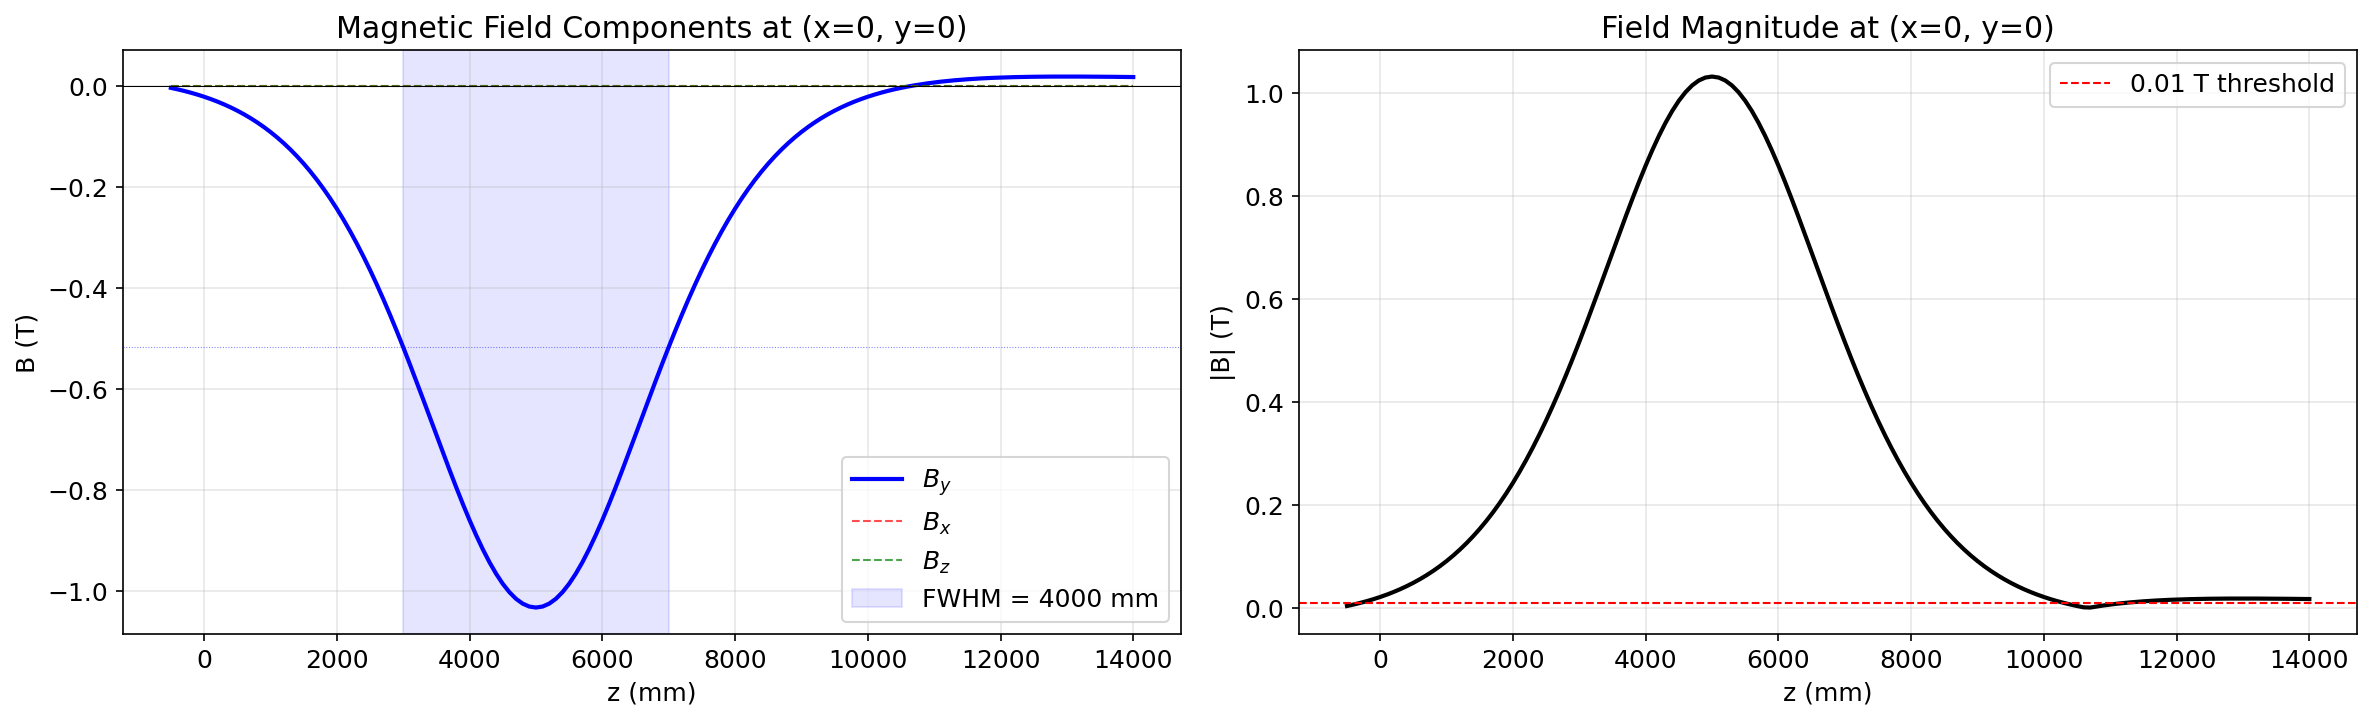
\includegraphics[width=\textwidth]{figures/field_By_z_profile.png}
\caption{Left: field components at $(x,y) = (0,0)$. $B_y$ dominates;
$B_x$ and $B_z$ are consistent with zero on-axis.
Right: field magnitude with 0.01\,T threshold defining the active region.}
\label{fig:By_profile}
\end{figure}

\begin{table}[h]
\centering
\caption{On-axis field characteristics (from notebook output).}
\label{tab:char}
\begin{tabular}{lll}
\toprule
\textbf{Property} & \textbf{Value} & \textbf{Significance for Cost Function} \\
\midrule
Peak $B_y$   & $-1.032$\,T at $z = 5000$\,mm & Sets maximum $\mathrm{d}t_x/\mathrm{d}z$ \\
FWHM         & 4000\,mm ($z \in [3000, 7000]$) & Field-active region for $t_x$ learning \\
$\int |B_y|\,\mathrm{d}z$ & 4544\,T$\cdot$mm & Determines $\Delta t_x$ magnitude \\
Central 98\% & $z \in [900, 11\,400]$\,mm & Minimum training $z$-range \\
Active region & $z \in [-300, 14\,000]$\,mm & $|B| > 0.01$\,T \\
Polarity     & $B_y < 0$ (MagDown) & Bends $x$ positively for $q > 0$ \\
\bottomrule
\end{tabular}
\end{table}

%======================================================================
\section{2D Field Structure}
\label{sec:2d}
%======================================================================

Figure~\ref{fig:2d_slices} shows $(x,z)$ and $(y,z)$ slices of all
three components.

\begin{figure}[ht]
\centering
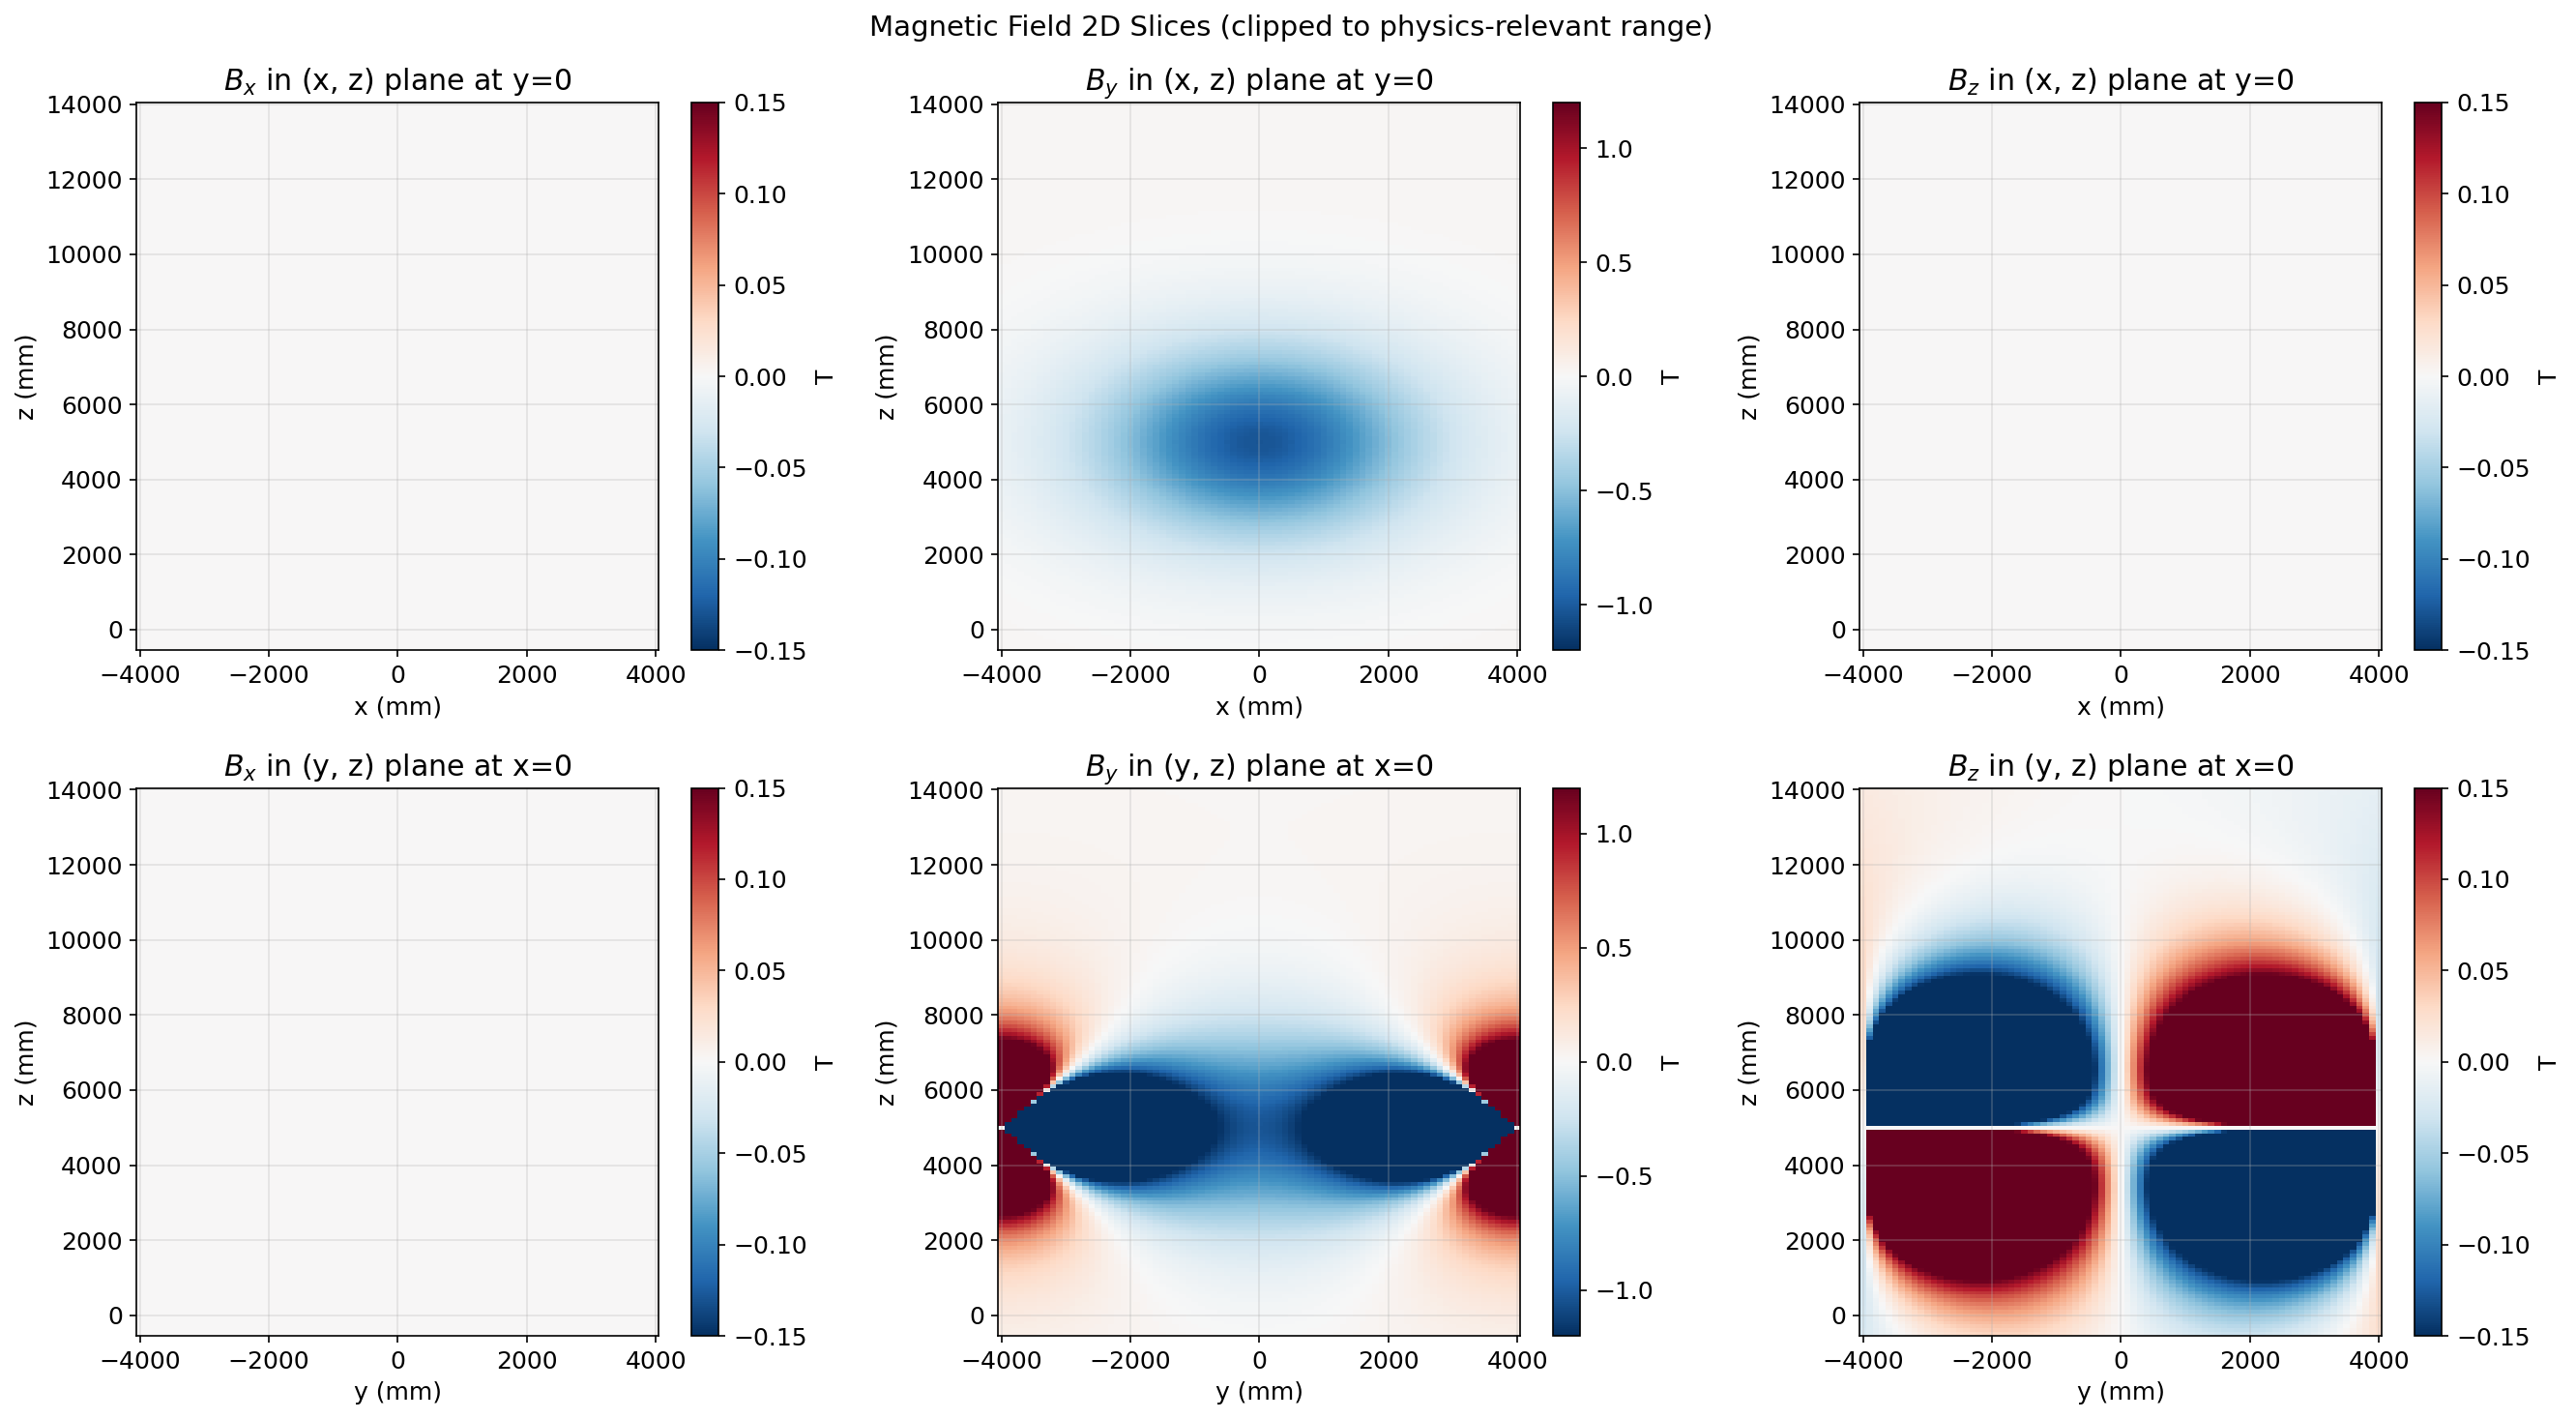
\includegraphics[width=\textwidth]{figures/field_2d_slices.png}
\caption{2D field slices (clipped to physics-relevant range).
Top: $(x,z)$ plane at $y = 0$. Bottom: $(y,z)$ plane at $x = 0$.
$B_y$ is the dominant component with a localised peak.
$B_x$ and $B_z$ show antisymmetric fringe patterns.}
\label{fig:2d_slices}
\end{figure}

Key observations:
\begin{itemize}[leftmargin=*]
  \item $B_y$ is approximately \emph{symmetric} in both $x$ and $y$.
  \item $B_x$ is \emph{antisymmetric} in $y$ and small ($< 0.15$\,T).
  \item $B_z$ is \emph{antisymmetric} in $x$ and small ($< 0.15$\,T).
  \item The fringe components $B_x$ and $B_z$ are responsible for the
        (small) changes in $t_y$; their antisymmetric structure means
        the \emph{sign} of $\delta t_y$ depends on the track's $(x,y)$
        position.
\end{itemize}

%======================================================================
\section{Transverse Variation: The 14\% Problem}
\label{sec:transverse}
%======================================================================

Figure~\ref{fig:transverse} shows how $B_y$ varies with $x$ and $y$ at
the peak $z$.

\begin{figure}[ht]
\centering
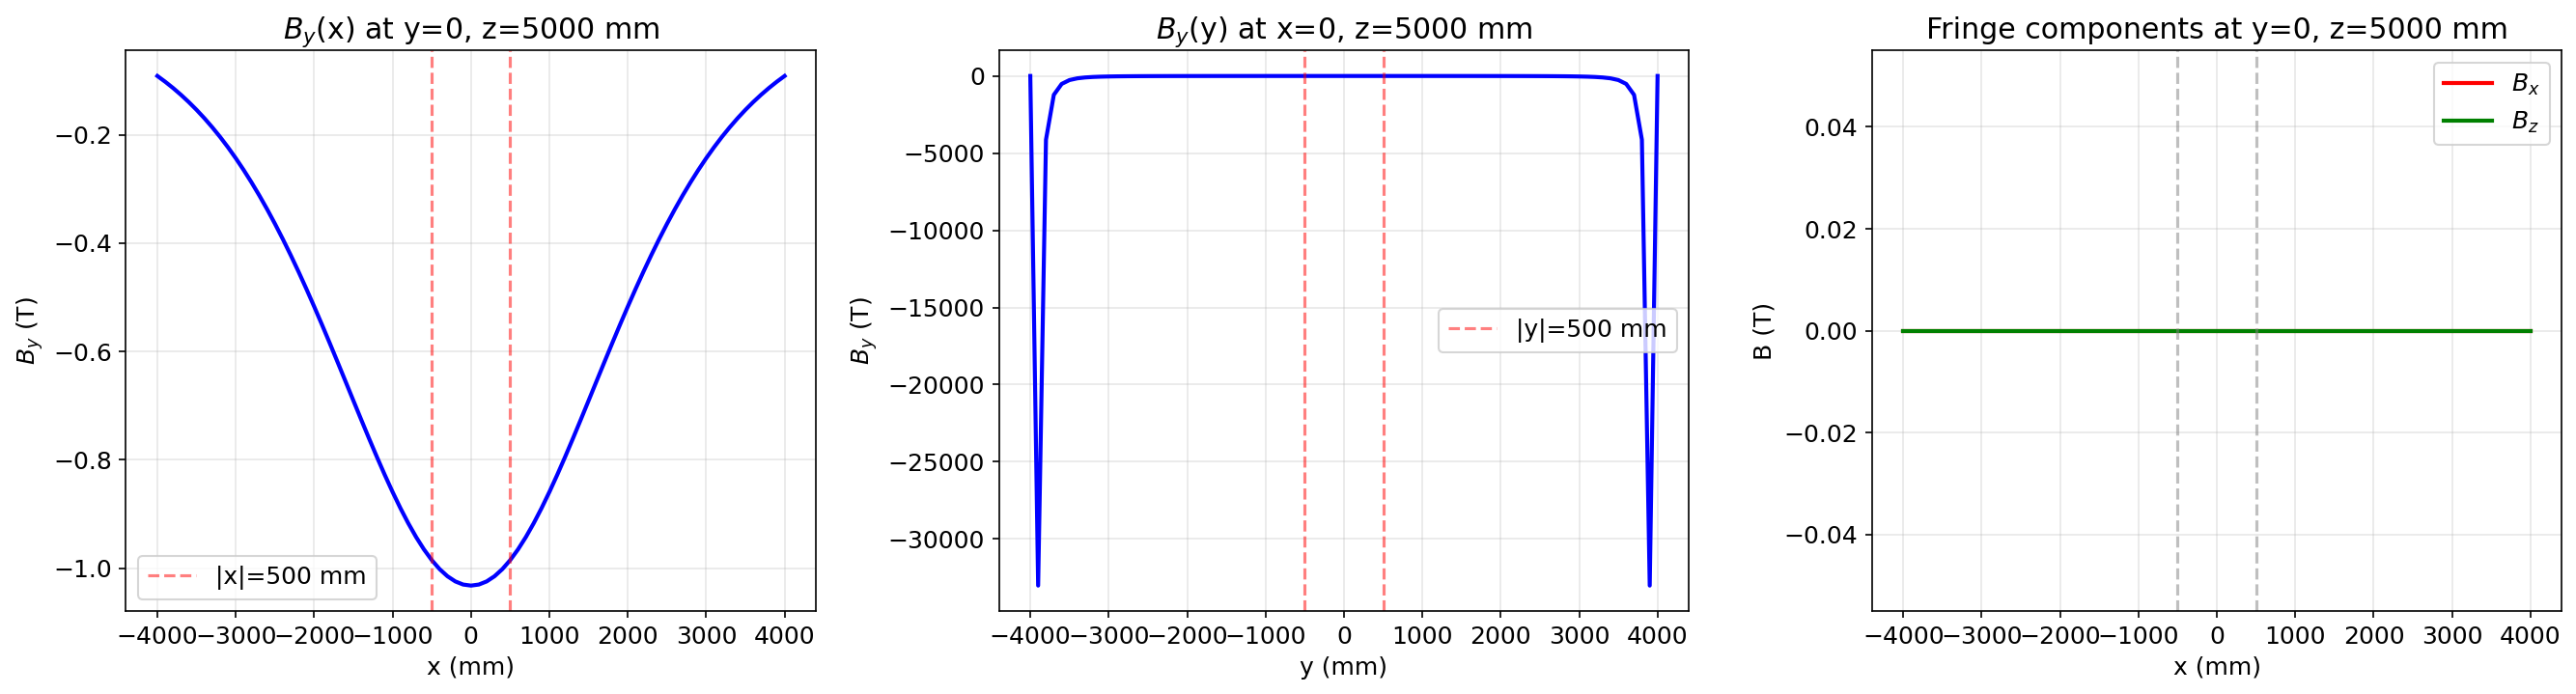
\includegraphics[width=\textwidth]{figures/field_transverse_variation.png}
\caption{Left/centre: $B_y$ vs $x$ and $y$ at $z = 5000$\,mm.
Right: fringe components $B_x$ and $B_z$ vs $x$.
Red dashed lines mark $|x|,|y| = 500$\,mm acceptance.}
\label{fig:transverse}
\end{figure}

Within the acceptance ($|x|, |y| < 500$\,mm):
\begin{itemize}[leftmargin=*]
  \item $B_y$ ranges from $-1.133$ to $-0.985$\,T (14.3\% relative variation).
  \item This is \textbf{not negligible}. A model that treats $B_y$ as
        $z$-only (Gaussian approximation) incurs a systematic position-dependent
        error in $\Delta t_x$ of up to 14\%.
\end{itemize}

\textbf{Critical implication}: The ML model \emph{must} receive the track's
$(x, y)$ position as input, not just $z$, because the field integral a
track experiences depends on where it is transversely.
A model that only takes $(t_x, t_y, q/p, z_{\text{in}}, \Delta z)$ as
inputs will systematically mispredict $\Delta t_x$ for off-axis tracks.

%======================================================================
\section{Gaussian Approximation: 12.6\,mT Systematic}
\label{sec:gaussian}
%======================================================================

The commonly used analytical approximation is
\begin{equation}
B_y(z) = B_0 \exp\!\Bigl[-\tfrac{1}{2}
  \Bigl(\frac{z - z_c}{z_w}\Bigr)^{\!2}\Bigr] ,
\quad B_x = B_z = 0 ,
\end{equation}
with fitted parameters $B_0 = -1.015$\,T, $z_c = 5000$\,mm,
$z_w = 1757$\,mm.

Figure~\ref{fig:gaussian_comparison} shows the comparison.

\begin{figure}[ht]
\centering
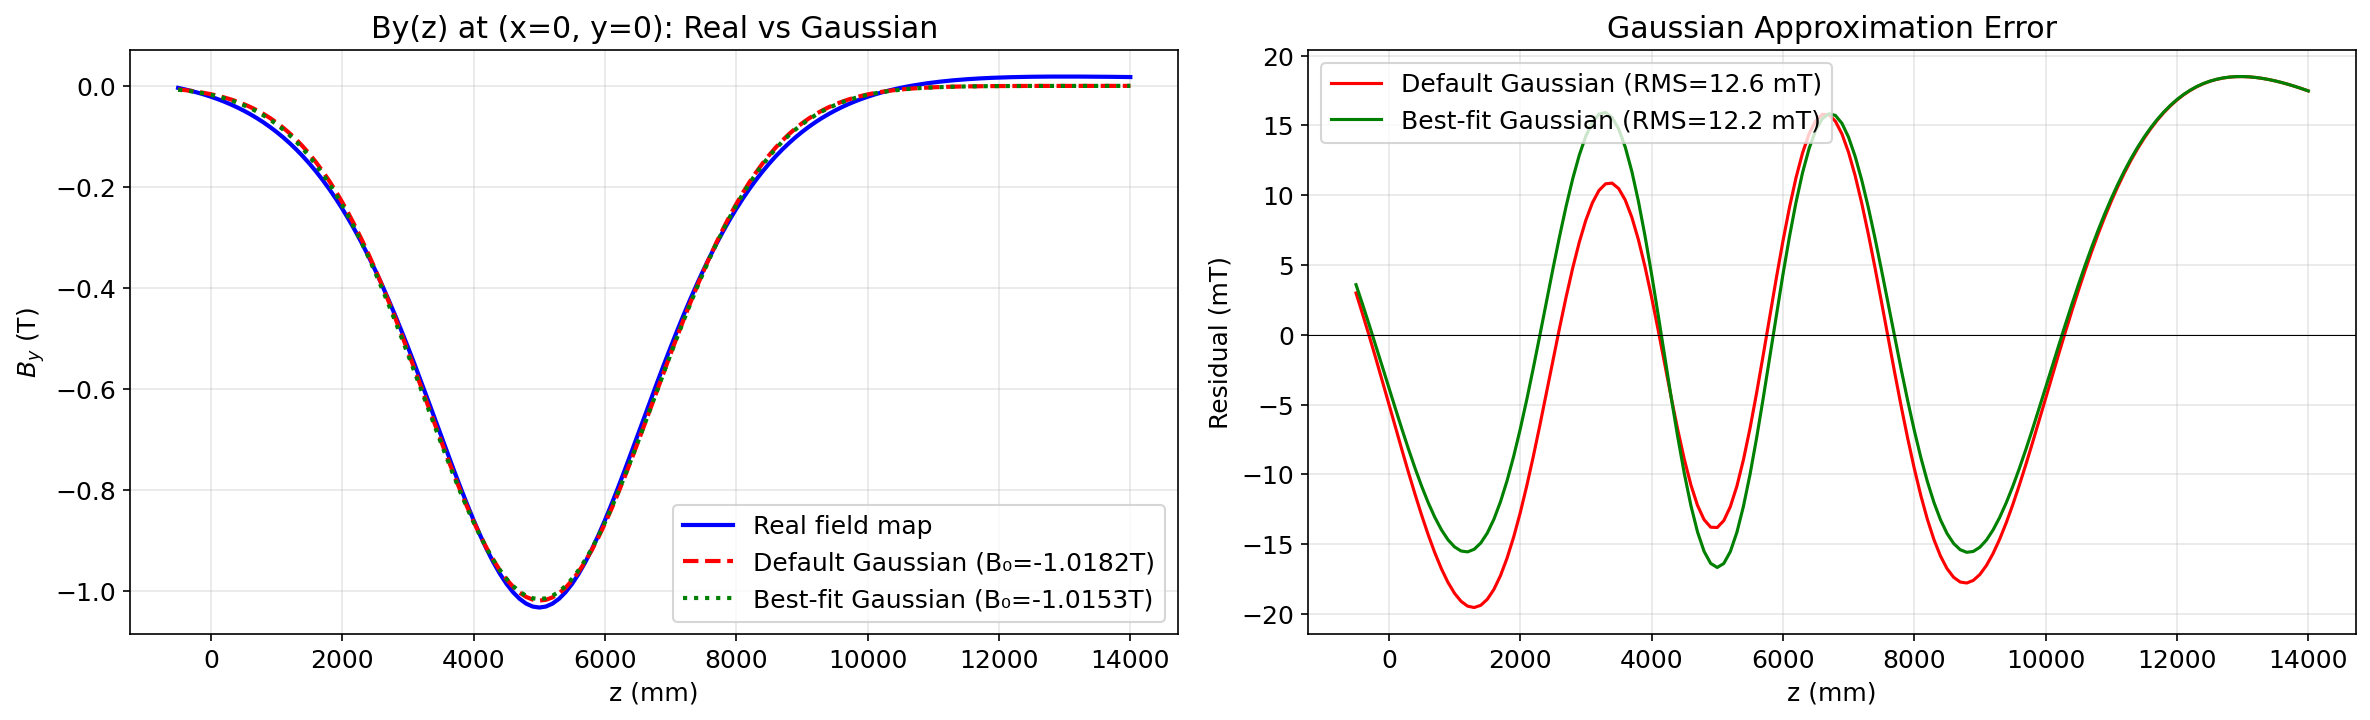
\includegraphics[width=\textwidth]{figures/field_gaussian_comparison.png}
\caption{Left: on-axis $B_y$ from the field map vs two Gaussian fits.
Right: residuals. The Gaussian misses the asymmetric tails of the real field.}
\label{fig:gaussian_comparison}
\end{figure}

\begin{table}[h]
\centering
\caption{Gaussian approximation error budget.}
\label{tab:gauss_error}
\begin{tabular}{lll}
\toprule
\textbf{Error Source} & \textbf{Magnitude} & \textbf{Effect on State} \\
\midrule
RMS $B_y$ error (on-axis)      & 12.6\,mT (1.2\%) & $\delta(\Delta t_x) \sim 1.2\%$ \\
Max $B_y$ error (on-axis)      & 19.5\,mT          & At tails ($z < 2000$, $z > 8000$) \\
$B_x, B_z$ omission            & up to $\sim 0.1$\,T & $\delta t_y$ entirely missing \\
Transverse $(x,y)$ variation   & 14.3\%             & Position-dependent $\Delta t_x$ bias \\
\bottomrule
\end{tabular}
\end{table}

\textbf{Verdict}: The Gaussian approximation introduces at least 3 distinct systematics.
For the ML extrapolator, training data \emph{must} be generated with the
trilinear-interpolated field map (or the C++ \texttt{MagneticFieldGrid}),
never the Gaussian.

\textbf{However}, the Gaussian can be useful as a \emph{physics-informed
loss regulariser}: evaluating $\mathrm{d}t_x/\mathrm{d}z \approx
(q/p)\,n\,B_y^{\text{Gauss}}(z)$ as a soft constraint costs zero field
lookups and guides the network toward the correct functional form, even
if it introduces a $\sim 1\%$ bias that the data term corrects.

%======================================================================
\section{Training $z$-Range}
\label{sec:zrange}
%======================================================================

Figure~\ref{fig:zrange} shows the cumulative field integral and
recommended training ranges.

\begin{figure}[ht]
\centering
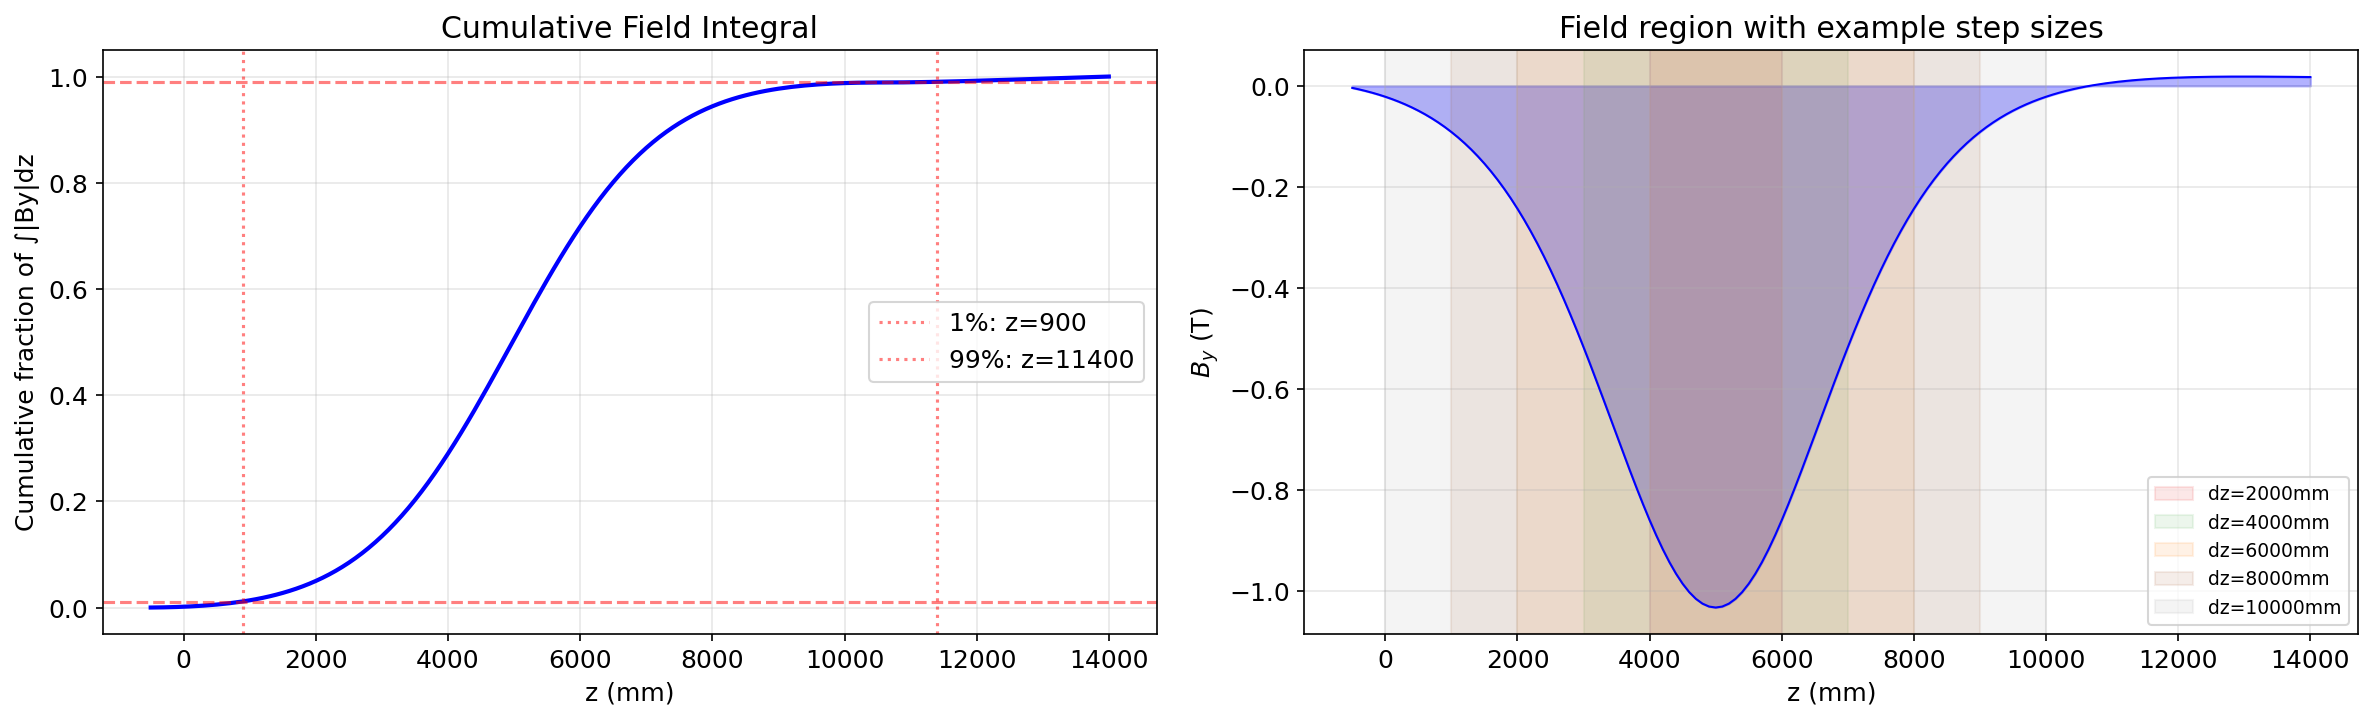
\includegraphics[width=\textwidth]{figures/field_z_range_recommendation.png}
\caption{Left: cumulative fraction of $\int |B_y|\,\mathrm{d}z$.
Right: $B_y(z)$ with example step sizes centred on the peak.}
\label{fig:zrange}
\end{figure}

The 1\%--99\% integral range is $z \in [900, 11\,400]$\,mm.
Training data should cover at least this range, with dense sampling
in the FWHM region $z \in [3000, 7000]$\,mm where $\Delta t_x$
changes most rapidly.

%======================================================================
\section{Physics of State--Field Coupling}
\label{sec:physics}
%======================================================================

\subsection{Equations of Motion}

The track state is $\mathbf{s} = (x, y, t_x, t_y, q/p)$ at position $z$.
The Lorentz force gives (see \texttt{ExtrapolatorCommon.cuh}):
\begin{align}
\frac{\mathrm{d}x}{\mathrm{d}z} &= t_x , \label{eq:dx} \\
\frac{\mathrm{d}y}{\mathrm{d}z} &= t_y , \label{eq:dy} \\
\frac{\mathrm{d}t_x}{\mathrm{d}z} &= \frac{q}{p}\,n\,
  \bigl[t_y(t_x B_x + B_z) - (1 + t_x^2)\,B_y\bigr] , \label{eq:dtx} \\
\frac{\mathrm{d}t_y}{\mathrm{d}z} &= \frac{q}{p}\,n\,
  \bigl[(1 + t_y^2)\,B_x - t_x(t_y B_y + B_z)\bigr] , \label{eq:dty} \\
\frac{\mathrm{d}(q/p)}{\mathrm{d}z} &= 0 , \label{eq:dqop}
\end{align}
with $n = \sqrt{1 + t_x^2 + t_y^2}$.

\subsection{Hierarchy of Scales}

Given the measured field properties, we can estimate the magnitude of
each derivative at the field peak for a 10\,GeV/$c$ track with
$t_x = t_y = 0.1$, $q/p \approx 3 \times 10^{-5}$\,MeV$^{-1}$:

\begin{table}[h]
\centering
\caption{Order-of-magnitude derivatives at the field peak.}
\label{tab:hierarchy}
\begin{tabular}{lllll}
\toprule
\textbf{Derivative} & \textbf{Dominant $B$ term} & \textbf{Order at 10\,GeV} & \textbf{$\times \Delta z$} & \textbf{Ratio to $\Delta x$} \\
\midrule
$\mathrm{d}x/\mathrm{d}z = t_x$
  & --- & $\sim 0.1$       & $\sim 800$\,mm & 1 \\
$\mathrm{d}y/\mathrm{d}z = t_y$
  & --- & $\sim 0.1$       & $\sim 800$\,mm & 1 \\
$\mathrm{d}t_x/\mathrm{d}z$
  & $(q/p)\,n\,B_y$ & $\sim 3 \times 10^{-5}$\,mm$^{-1}$
  & $\sim 0.24$   & $3 \times 10^{-4}$ \\
$\mathrm{d}t_y/\mathrm{d}z$
  & $(q/p)\,n\,B_x$ & $\sim 3 \times 10^{-7}$\,mm$^{-1}$
  & $\sim 0.002$  & $3 \times 10^{-6}$ \\
$\mathrm{d}(q/p)/\mathrm{d}z$
  & --- & \textbf{exactly 0} & 0 & 0 \\
\bottomrule
\end{tabular}
\end{table}

The dynamic range spans \textbf{6 orders of magnitude}, from $\Delta x
\sim 800$\,mm down to $\delta t_y \sim 0.002$.

\subsection{Why This Hierarchy Breaks Naive MSE Training}

Consider a naive cost function $\mathcal{L} = \mathrm{MSE}(\hat{\mathbf{s}},
\mathbf{s})$ over the 5-element output state:
\[
  \mathcal{L} = \frac{1}{5}\bigl[
    (\hat{x} - x)^2 + (\hat{y} - y)^2 + (\hat{t}_x - t_x)^2
    + (\hat{t}_y - t_y)^2 + (\widehat{q/p} - q/p)^2
  \bigr] .
\]
\begin{enumerate}[leftmargin=*]
  \item \textbf{$x$ dominates the loss}: With $|\Delta x| \sim 800$\,mm, even
        a 0.1\% relative error gives $(0.8\,\mathrm{mm})^2 = 0.64$.
        Meanwhile, a 100\% error on $\delta t_y \sim 0.002$ gives
        $(0.002)^2 = 4 \times 10^{-6}$.
        The optimiser will devote nearly all gradient signal to $x$
        and ignore $t_y$ entirely.
  \item \textbf{$t_x$ is underweighted}: The momentum-sensitive bending
        signal $\Delta t_x \sim 0.24$ contributes
        $\sim (0.024)^2 \approx 6 \times 10^{-4}$ at 10\% error---three
        orders of magnitude below $x$.
        \emph{The model can achieve a low total loss while completely
        ignoring the bending physics.}
  \item \textbf{$q/p$}: Since $q/p$ is constant, the naive model will
        learn to reproduce the input value for zero loss.
        This is trivially correct but wastes network capacity.
  \item \textbf{Momentum dependence of target scales}: At $p = 3$\,GeV/$c$,
        $\Delta t_x \sim 0.8$; at $p = 100$\,GeV/$c$,
        $\Delta t_x \sim 0.007$.
        A single global MSE loss is inappropriately weighted across
        the momentum spectrum.
\end{enumerate}

%======================================================================
\section{Recommended Cost Function Design}
\label{sec:cost}
%======================================================================

\subsection{Per-Element Target Transformations}

Based on the physics analysis above, each state element should have its
own transformed target and loss weight:

\begin{table}[ht]
\centering
\caption{Per-element target design.}
\label{tab:targets}
\renewcommand{\arraystretch}{1.3}
\begin{tabular}{lp{5.5cm}lp{4.5cm}}
\toprule
\textbf{Element} & \textbf{Target (what to predict)} & \textbf{Scale} & \textbf{Justification} \\
\midrule
$x$ &
$\delta x = x_{\mathrm{out}} - (x_{\mathrm{in}} + t_{x,\mathrm{in}} \cdot \Delta z)$
\newline (deflection from straight line)
& $\sim\! 0$--$30$\,mm & Removes the large kinematic $t_x \Delta z$ term.
Residual is pure field effect, $\propto q/p$. \\
\midrule
$y$ &
$\delta y = y_{\mathrm{out}} - (y_{\mathrm{in}} + t_{y,\mathrm{in}} \cdot \Delta z)$
& $\sim\! 0$--$0.5$\,mm & Nearly linear; ML target is small correction only. \\
\midrule
$t_x$ &
$\Delta t_x = t_{x,\mathrm{out}} - t_{x,\mathrm{in}}$
\newline (slope change)
& $[-0.8, +0.8]$ & Direct measure of $\int (q/p)\,B_y\,\mathrm{d}z$;
\textbf{the key physics signal}. \\
\midrule
$t_y$ &
$\Delta t_y = t_{y,\mathrm{out}} - t_{y,\mathrm{in}}$
& $\sim\! O(10^{-3})$ & Small; driven by fringe $B_x, B_z$.
Can be dropped in first iteration. \\
\midrule
$q/p$ &
Do \textbf{not} predict.
& --- & Exact invariant of motion.
Use a skip connection: $\widehat{q/p} = q/p_{\mathrm{in}}$. \\
\bottomrule
\end{tabular}
\end{table}

\subsection{Recommended Loss Function}

\begin{equation}
\boxed{
\mathcal{L} =
  w_x \cdot \mathrm{MSE}(\widehat{\delta x},\, \delta x)
+ w_y \cdot \mathrm{MSE}(\widehat{\delta y},\, \delta y)
+ w_{t_x} \cdot \mathrm{MSE}(\widehat{\Delta t_x},\, \Delta t_x)
+ w_{t_y} \cdot \mathrm{MSE}(\widehat{\Delta t_y},\, \Delta t_y)
}
\label{eq:loss}
\end{equation}

\noindent
where the weights $w_i$ are chosen to \emph{equalise gradient magnitudes}
across elements.  In practice this means normalising each target to
unit variance over the training set and setting $w_i = 1/\sigma_i^2$.

\subsection{Physics-Informed Regularisation}

An optional but powerful extension adds an ODE-consistency loss:
\begin{equation}
\mathcal{L}_{\mathrm{ODE}} =
  \lambda \cdot \Bigl\|
    \frac{\widehat{\Delta t_x}}{\Delta z}
    - \frac{q}{p}\,n\,B_y\bigl(x_{\mathrm{mid}}, y_{\mathrm{mid}}, z_{\mathrm{mid}}\bigr)
  \Bigr\|^2 ,
\label{eq:ode_loss}
\end{equation}
where the midpoint $(x_{\mathrm{mid}}, y_{\mathrm{mid}}, z_{\mathrm{mid}})$
is estimated from the predicted state.  Key considerations:
\begin{itemize}[leftmargin=*]
  \item This penalises curvature predictions inconsistent with the
        known Lorentz equation, without requiring additional training data.
  \item The Gaussian field approximation can be used for $B_y$ in this
        term (avoiding field lookups), accepting a $\sim 1.2\%$ systematic
        that the data term will correct.
  \item The regularisation coefficient $\lambda$ should be small enough
        not to override data-driven learning, but large enough to prevent
        unphysical solutions in low-data regions.
  \item \textbf{Caveat}: This term only constrains $t_x$.  Adding an
        analogous term for $t_y$ requires $B_x$ evaluation (non-trivial
        on GPU).
\end{itemize}

\subsection{Multiplicative Architecture for $\Delta t_x$}

Since $\Delta t_x \propto q/p$ (linearly), a natural architecture choice is:
\begin{equation}
\widehat{\Delta t_x} = \frac{q}{p} \cdot f_\theta(t_x, t_y, x, y, z_{\mathrm{in}}, \Delta z) ,
\end{equation}
where $f_\theta$ is a small MLP that learns only the geometry-dependent
field integral.  This:
\begin{itemize}[leftmargin=*]
  \item Guarantees $\Delta t_x = 0$ when $q/p = 0$ (straight track).
  \item Immediately captures the correct momentum scaling, so the
        network doesn't waste capacity learning a linear relationship.
  \item Reduces relative error at high $p$ (where $\Delta t_x$ is small
        and otherwise lost in the loss).
\end{itemize}

Similarly, $\delta x$ should use a
$\widehat{\delta x} = (q/p) \cdot g_\theta(\ldots)$ structure, since
the horizontal deflection is also proportional to $q/p$.

%======================================================================
\section{Summary of Field-Driven Constraints}
\label{sec:summary}
%======================================================================

\begin{table}[ht]
\centering
\caption{Field properties and their direct constraints on the ML model.}
\label{tab:summary}
\renewcommand{\arraystretch}{1.15}
\begin{tabular}{p{4.5cm}lp{5.5cm}}
\toprule
\textbf{Field Property} & \textbf{Value} & \textbf{ML Constraint} \\
\midrule
Peak $|B_y|$ = 1.032\,T & at $z = 5000$\,mm &
  Max $\mathrm{d}t_x/\mathrm{d}z$; sets scale of $\Delta t_x$ target \\
FWHM = 4000\,mm & $z \in [3000, 7000]$ &
  Dense training sampling needed here \\
$\int |B_y|\,\mathrm{d}z = 4544$\,T$\cdot$mm & -- &
  $\Delta t_x \sim (q/p) \times 4544$; determines target range \\
Transverse variation 14.3\% & within $|x,y| < 500$\,mm &
  Model \emph{must} take $(x,y)$ as inputs \\
$B_x, B_z < 0.15$\,T & antisymmetric fringe &
  $\Delta t_y$ is small and position-dependent \\
Gaussian RMS error 12.6\,mT & 1.2\% &
  Cannot use for data gen; acceptable for physics loss \\
Edge artefacts $|B| > 33\times10^3$\,T & at $|y| = 4000$\,mm &
  Must clamp or mask grid edges \\
$q/p$ invariance & exact &
  Skip connection; do not learn \\
6 OoM dynamic range in $|\mathrm{d}s_i/\mathrm{d}z|$ & -- &
  Per-element loss normalisation is mandatory \\
\bottomrule
\end{tabular}
\end{table}

\subsection{Things That Will Go Wrong Without This Analysis}

\begin{enumerate}[leftmargin=*]
  \item \textbf{No residual targets}: Loss dominated by kinematic $t_x
        \Delta z$ term. Model learns a straight-line extrapolator and
        plateaus.
  \item \textbf{No loss weighting}: $\Delta t_x$ gradients are
        $10^3 \times$ smaller than $x$ gradients. Model achieves low loss
        by fitting $x$ and ignoring the bending physics.
  \item \textbf{$z$-only input}: 14\% position-dependent field systematic
        permanently baked in.
  \item \textbf{Un-masked grid}: A single $|B| = 33\,000$\,T artefact
        point destroys training.
  \item \textbf{Learning $q/p$}: Network wastes capacity on identity
        function; covariance structure confused during Kalman update.
  \item \textbf{Flat $p$ sampling}: Low-$p$ tracks (large $\Delta t_x$)
        dominate loss; high-$p$ tracks (small $\Delta t_x$) are never learned.
        Use log-uniform $p$ sampling.
\end{enumerate}

\end{document}
